\chapter{Entwicklung des eingebetteten Systems}
Damit der Rollstuhl-Software bekannt ist, mit welcher Geschwindigkeit sich welches Rad in welche Richtung dreht, ist Hardware notwendig.
Um dies zu bewerkstelligen wurde ein eingebettetes System entwicklet. Dieses muss die Rotationsdaten messen und an die Software übermitteln.
Dabei kommt ein ESP32-Mikrocontroller zum Einsatz, der ein Gyroskop ausliest und anschließend die Daten mithilfe eines Übertragungsprotokolls an die Rollstuhl-Software überträgt.
Näher soll in einem Vergleich beleuchtet werden, ob die Protokolle WiFi und ESP-Now für den vorliegenden Anwendungsfall geeignet sind.

\section{PlatformIO}
Zur Entwicklung der eingebetteten Software, die auf den Mikrocontrollern läuft, wurde PlatformIO verwendet.
Dies ist eine Framework-Erweiterung für Visual Studio Code, bei der die benötigten Bibliotheken, die für jeden Mikrocontroller und jedes Board notwendig sind, automatisch heruntergeladen und eingerichtet werden\cite{WhatPlatformIOPlatformIO}.
Ebenfalls lassen sich über das \ac{ui}, Bibliotheken, die für das jeweilige Projekt notwendig sind, hinzufügen.
Zusätzlich zur Entwicklungsumgebung von Visual Studio Code gibt es Funktionalitäten einen Chip zu flashen und anschließend im seriellen Monitor die Ausführung zu beobachten.
Im Gegensatz zu Umgebungen wie der Arduino \ac{ide} wird Zeit gespart, da dort zunächst manuell Treiber heruntergeladen werden müssen.
Zusätzlich kann man nicht von den Vorteilen einer modernen \ac{ide} profitieren.

\section{Messung der Raddaten}
Um die Rotation der Räder des Rollstuhls messen zu können, wird ein Sensor benötigt.
Dabei wurde sich für ein Gyroskop entschieden, da diese verfügbar, kostengünstig und leicht integrierbar sind\footnote{Es wurde sich gegen die Verwendung einer Lichtschranke entschieden, da bei dieser Art von Messung keine kleinen Geschwindigkeiten möglich sind.}.
Jedoch erfordert die Verwendung eines Gyroskops eine Voreinstellung und Kalibrierung, welche in diesem Unterkapitel erörtert werden sollen.

\subsection{Gyroskop}
Im Zuge dieser Arbeit wurde sich für das Motion-Tracking-Device GY-521 MPU-6050 entschieden.
Dieses ist klein (mit Pins: 20mm x 15mm x 11mm), kostengünstig zu erwerben (ca. 4 Euro) und verfügt unter anderem über 3-Achsen-Gyroskop-Sensoren, mit denen die Rotation gemessen werden kann.
Der Chip besitzt folgende 8 Anschlüsse:

\begin{table}[h]
    \centering
    \begin{threeparttable}
        \caption{Pins des GY-521 MPU-6050\cite{az-delivery_vertriebs_gmbhGY5216AchsenGyroskop}}
        \begin{tabular}{|l|l|l|}
            \hline
            \textbf{Anschluss}          & \textbf{Funktion}        & \textbf{Notwendig} \\ \hline
            \parbox[c][0.5cm]{2cm}{VCC} & Power-Supply             & Ja                 \\ \hline
            \parbox[c][0.5cm]{2cm}{GND} & Ground                   & Ja                 \\ \hline
            \parbox[c][0.5cm]{2cm}{SCL} & I2C Serial-Clock Line    & Ja                 \\ \hline
            \parbox[c][0.5cm]{2cm}{SDA} & I2C Serial-Date Line     & Ja                 \\ \hline
            \parbox[c][0.5cm]{2cm}{XDA} & Auxiliary Serial Data    & Nein               \\ \hline
            \parbox[c][0.5cm]{2cm}{XCL} & Auxiliary Serial Clock   & Nein               \\ \hline
            \parbox[c][0.5cm]{2cm}{ADO} & I2C Address Select       & Ja                 \\ \hline
            \parbox[c][0.5cm]{2cm}{INT} & Interrupt Digital Output & Nein               \\ \hline
        \end{tabular}
    \end{threeparttable}
\end{table}

Die Daten können mithilfe eines angeschlossenen Mikrocontrollers (ESP32) ausgelesen werden.
Jede Achse wird auf zwei 8-Bit-Register abgebildet\cite{invensenseinc.MPU6000MPU6050Register2013}.
Zusammen ergibt das einen Wertebereich von 65.536 unterscheidbaren Zuständen.
Mit der Drehrichtung rückwärts halbiert sich dieser Wertebereich, da ein Bit für das Verschieben des Wertebereichs ins Negative benötigt wird.
Das Gyroskop des MPU-6050 kann in vier verschiedenen Konfigurationen betrieben werden\cite{invensenseinc.MPU6000MPU6050Register2013}.
Damit wird festgelegt, wie klein der Winkel zwischen zwei verschiedenen Zuständen ist; mit anderen Worten, wie viele Stufen pro Grad unterschieden werden können.
Da der Wertebereich konstant ist, bedeutet eine empfindlichere Messung, dass das Gyroskop bei einer geringeren Geschwindigkeit das Ende des Wertebereichs erreicht.
Angewendet auf den Rollstuhl hat das zur Folge, dass das rotierende Rad bei niedrigeren Geschwindigkeiten seine maximal messbare Geschwindigkeit erreicht.
Es gilt folgender Zusammenhang mit welchem die aktuelle Winkelgeschwindigkeit errechnet werden kann:

\begin{align}
    z        & : \ \mathrm{Gemessene\ Stufen}\ [\si{1/\second}]                                \\
    z_m      & : \ \mathrm{Maximale\ Anzahl\ von\ Stufen}\ [\si{1/\second}]                    \\
    p        & : \ \mathrm{Stufen\ pro\ Grad}\ [\si{1/\degree}]                                \\
    \omega   & : \ \mathrm{Aktuelle\ Winkelgeschwindigkeit}\ [\si{\degree/\second}]            \\
    \omega_m & : \ \mathrm{Maximal\ messbarere\ Winkelgeschwindigkeit}\ [\si{\degree/\second}]
\end{align}

\begin{align}
    z_m    & = \pm 32768                  \\
    z_m    & = \omega_m \cdot p           \\
    \omega & = \left(\frac {z} {p}\right)
\end{align}

\begin{table}[h]
    \centering
    \begin{threeparttable}
        \caption{Einstellbare Modi des Gyroskops mit ihren resultierenden Eigenschaften}
        \begin{tabular}{|l|l|l|l|l|}
            \hline
            ~ & \textbf{Modus 0} & \textbf{Modus 1} & \textbf{Modus 2} & \textbf{Modus 3} \\ \hline
            \parbox[c][1.5cm]{4cm}{\textbf{Maximal messbarere                             \\Winkel-\\geschwindigkeit [\si{\degree/\second}]*}}  & 250     & 500     & 1000    & 2000    \\ \hline
            \parbox[c][1cm]{4cm}{\textbf{Stufen                                           \\pro Grad [\si{\second/\degree}]*}}                  & 131     & 65,5    & 32,8    & 16,4    \\ \hline
            \parbox[c][1.5cm]{4cm}{\textbf{Maximale                                       \\Umdrehungszahl \\pro Sekunde [\si{1/\second}]}}     & 0,69    & 1,39    & 2,78    & 5,56    \\ \hline
            \parbox[c][1cm]{4cm}{\textbf{Maximale Radianten                               \\pro Sekunde [\si{\radian/\second}]}}                & 4,36    & 8,73    & 17,47   & 34,93   \\ \hline
            \parbox[c][1cm]{4cm}{\textbf{Zurückgelegte Distanz                            \\pro Stufe [\si{\milli\metre}]**}}                   & 0,04    & 0,08    & 0,16    & 0,32    \\ \hline
        \end{tabular}
        \begin{tablenotes}
            \small
            \item
            *\cite{invensenseinc.MPU6000MPU6050Register2013}\\ **Werte bei einem Raddurchmesser von 60 cm
        \end{tablenotes}
    \end{threeparttable}
\end{table}

Es stellt sich die Frage, welcher der optimale Modus für das hier entwickelte System ist.
Um dem Nutzer ein möglichst störungsfreies Erlebnis zu bieten, muss gewährleistet sein, dass das Gyroskop so empfindlich wie möglich eingestellt ist.
Das bedeutet, dass der Wertebereich maximal ausgereizt werden muss.
Ist der Modus nicht empfindlich genug, so bemerkt der Nutzer möglicherweise das Springen der Bitwerte in Form eines Vorspringens in der Bewegung.
Allerdings muss ein Modus gewählt werden, welcher dazu führt, dass der Nutzer nicht schneller als die maximale Gradzahl pro Sekunde drehen kann, da es sonst zu einem Zahlenüberlauf kommt und zu einer fehlerhaften Weiterverarbeitung der Daten führt.
Der Zahlenüberlauf kann zwar abgefangen werden, jedoch sollte bei Bedarf einer maximale Geschwindigkeit diese programmgesteurert festgelegt werden.
Dies birgt den Vorteil den maximalen Wert flexibler setzen zu können.
Der Modus muss also so empfindlich sein, dass der Nutzer nicht den Übergang von einem Zustand in den nächsten registriert.
Gleichzeitig darf er nicht in der Lage sein, die Räder schneller als die maximale Gradzahl pro Sekunde zu drehen.

\subsection{Idealer Gyroskop-Modus}
Wie zuvor beschrieben, muss der Frage nachgegangen werden, in welchem Modus das Gyroskop betrieben werden sollte.
Hierfür wurde eine Datenreihe gemessen, mit der Gradzahl pro Sekunde im Verlauf der Zeit.
Eine Testperson hat dabei versucht, ein Rad so schnell wie möglich zu drehen.

\begin{figure}[h]
    \centering
    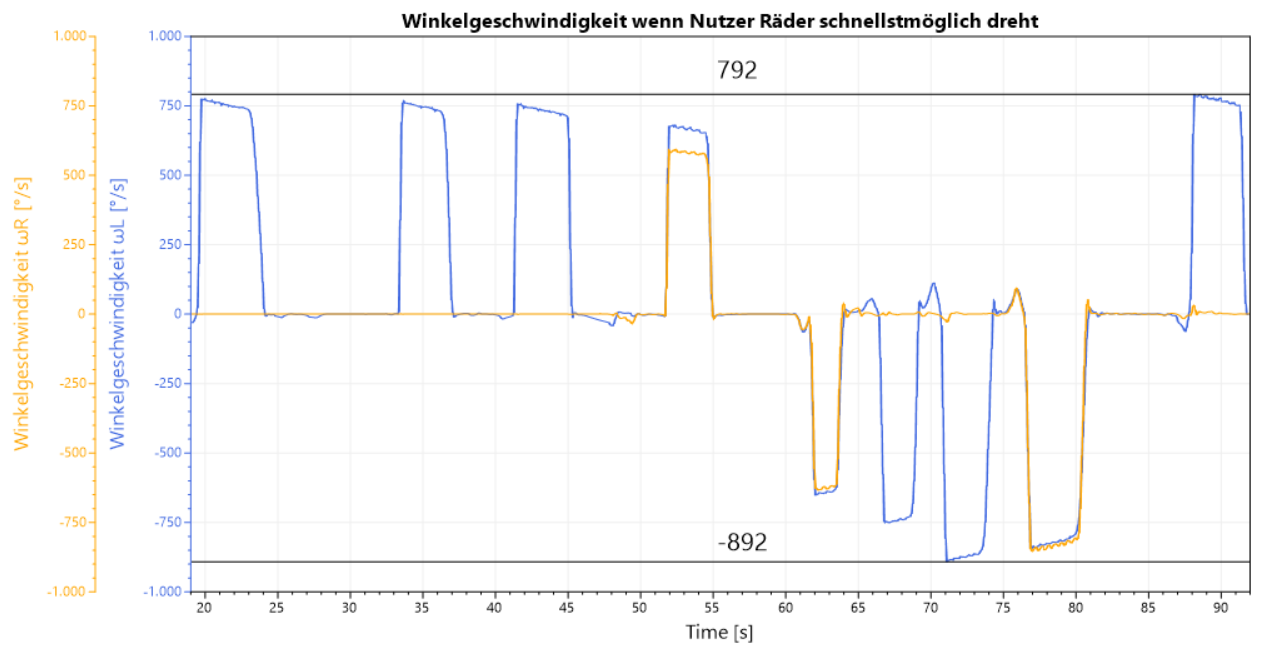
\includegraphics[width=\textwidth]{gyroMax.PNG}
    \caption{Winkelgeschwindigkeiten der Räder im Verlauf der Zeit, bei dem die Testperson ein Rad, mit der dominanten Hand, so schnell wie möglich dreht}
    \label{fig:gyroMax}
\end{figure}

Abbildung \ref{fig:gyroMax} zeigt bei einer Roation nach vorne einen maximal erreichten Ausschlag um $800\ \si{\degree}/s$.
Bei Rotationen nach hinten ist der Ausschlag etwas höher, übersteigt jedoch nicht $-900\ \si{\degree}/s$.
Daraus folgt, dass Gyroskop-Modus 2 für dieses Szenario der Ideale ist.
Bei diesem Modus ist die Maximale Gradzahl pro Sekunde $1000\ \si{\degree}/s$.
Der Nutzer erreicht nicht die maximal Geschwindigkeit und reizt trotzdem den Wertebereich ca. $80\ \%-90\ \%$ aus. Deshalb wird dieser Modus im System verwendet.

In vielen Anwendungen ist es von Vorteil oder angenehmer für den Nutzer, sich schnellstmöglich mit der maximalen Fortbewegungsgeschwindigkeit zu bewegen.
Auf Dauer ist es ermüdend, die Räder möglichst schnell drehen zu müssen.
Um den Nutzer zu entlasten, kann entweder der Fortbewegungsvektor $\vec{f}$ immer auf einen maximalen Thumbstick-Ausschlag abgebildet werden oder es wird ein weiterer Schwellenwert eingeführt, ab dem alle Eingaben als maximaler Thumbstick-Ausschlag abgebildet werden.

\subsection{Verbesserung der Rohdaten}
Die ausgelesenen Werte des Gyroskops sind nicht automatisch kalibriert.
Sie besitzen einen konstanten Offset. Deshalb muss beim Start des Systems eine Kalibrierungssequenz gestartet werden.
Diese errechnet aus einer Reihe ausgelesener Werte einen Mittelwert, der anschließend von allen zukünftigen Werten abgezogen wird.
Dazu dürfen die Räder nicht bewegt werden, da dies das Ergebnis der Kalibrierung unbrauchbar machen würde.

Darüber hinaus hat das Gyroskop-Signal ein Rauschen.
Bei hoher Umdrehungszahl ist das Rauschen irrelevant, da es nur einen kleinen Anteil der Gesamtrotation ausmacht.
Steht das Rad still, ist das Rauschen jedoch störend, da in diesem Fall nicht erkennbar ist, ob es tatsächlich stillsteht oder eine geringe Rotation gegeben ist.
Aus diesem Grund wird ein Schwellenwert bestimmt, welcher der Gyroskop-Wert überschreiten muss, um als Bewegung erkannt werden zu können.
Damit ist sichergestellt, dass es sich um eine tatsächliche Rotation handelt.

\section{ESP32}
Um den MPU-6050 betreiben und dessen Daten an die Rollstuhl-Software übermitteln zu können, wird ein Mikrocontroller-Board benötigt.
Es muss die entsprechenden Register auslesen und mittels drahtloser Kommunikation versenden.
Auf dem Markt ist eine große Anzahl von Produkten für die verschiedensten Anwendungsgebiete erhältlich.
Im Rahmen dieser Arbeit wurde der Mikrocontroller ESP32 verwendet, das aktuelle Modell der Firma \textit{Espressif}.
Boards mit diesem Chip sind kostengünstig (ca. 8 Euro).
Zudem ist der ESP32 mit WiFi (802.11 b/g/n), Bluetooth (v4.2) und ESP-Now Unterstützung ausgestattet\cite{ESP32Datasheet2022}.
Verbaut wurde ein Xtensa® 32-bit LX6 Mikroprozessor, mit 240MHz Taktfrequenz, 448 KB \ac{rom} und 520 KB \ac{sram}\cite{ESP32Datasheet2022}.
Als Entwicklungsboard wurde das ESP32 Dev Kit C V4 verwendet.

Der MPU-6050 muss wie folgt an das Entwicklungsboard angeschlossen werden:

\begin{table}[h]
    \centering
    \begin{threeparttable}
        \caption{Zuweisungs der jeweiligen Pins}
        \begin{tabular}{|l|l|}
            \hline
            \textbf{ESP32}                          & \textbf{MPU-6050}           \\ \hline
            \parbox[c][0.5cm]{3cm}{3.3V}            & \parbox[c][0.5cm]{3cm}{VCC} \\ \hline
            \parbox[c][0.5cm]{3cm}{GND}             & \parbox[c][0.5cm]{3cm}{GND} \\ \hline
            \parbox[c][0.5cm]{3cm}{GPIO22 (I2C CL)} & \parbox[c][0.5cm]{3cm}{SDA} \\ \hline
            \parbox[c][0.5cm]{3cm}{GPIO21 (I2C DA)} & \parbox[c][0.5cm]{3cm}{SCL} \\ \hline
            \parbox[c][0.5cm]{3cm}{ADO}             & \parbox[c][0.5cm]{3cm}{GND} \\ \hline
        \end{tabular}
    \end{threeparttable}
\end{table}

\section{3D gedruckte Box}
Damit Entwicklungsboard, Gyroskop und Akku zusammengehalten werden, geschützt sind und am Rad befestigt werden können, wird eine Box benötigt, die alle Komponenten aufnehmen kann und diese trägt.
Aufgrund dessen wurde – mithilfe von Blender – eine entsprechend seinen Anforderungen konstruierte Box entworfen und mittels 3D-Druckers gedrucht.

\section{Vergleich zwischen WiFi und ESP-Now}
Für die Übermittlung der Sensordaten an die Rollstuhl-Software auf einem \ac{pc}, stehen verschiedene Möglichkeiten zur Verfügung.
In dieser Arbeit sind zwei verschiedene Protokolle getestet worden: WiFi und ESP-Now. Die Protokolle müssen dabei leicht in das System integrierbar sein.
WiFi ist ein weit verbreiteter Standard, sodass entsprechende Bibliotheken schon existieren, um das Protokoll einbinden zu können\cite{WiFiArduinoReference}.
ESP-Now ist weniger verbreitet, da aber der Chip vom selben Hersteller kommt, existieren auch hier schon Bibliotheken, beziehungsweise ist die benötigte Bibliothek schon im Entwicklungspaket des Chips schon enthalten\cite{EspressifIoTDevelopment2022}.
Ein weiteres verfügbares Protokoll ist Bluetooth.
Jenes muss jedoch aufgrund des zeitlichen Rahmens dieser Arbeit, an anderer Stelle beleuchtet werden.

\subsection{WiFi und WebSockets}
WiFi ist eine Kommunikationstechnologie, die durch die WiFi-Alliance entstanden ist und bis heute von ihr gepflegt wird\cite{WhoWeAre}.
Sie ermöglicht drahtlose Kommunikation mit jedem Gerät, welches diese Technologie implementiert.
Inzwischen ist WiFi ein weit verbreiteter Standard, welcher von den meisten mobilen Geräten unterstützt wird\cite{DiscoverWiFiWiFi}.
Ein solches Gerät ist der ESP32.

Zunächst muss eine Verbindung zwischen dem ESP32 und dem lokalen Netzwerk mittels WiFi aufgebaut werden.
Damit die Zugangsdaten nicht fest in den Code geschrieben werden müssen, wird die Bibliothek \textit{WiFi Manager}\cite{tzapuWiFiManager2022} verwendet.
Diese baut selbstständig eine Verbindung mit einem Netzwerk auf, nachdem die Zugangsdaten über ein Gerät wie zum Beispiel einem Smartphone übergeben wurden.
Dazu wird ein Web-Konfigurations-Portal auf dem ESP32 gehostet, auf das ein nahes WiFi-fähiges Gerät zugreifen kann.

Für die eigentliche Übertragung der Daten können verschiedene Protokolle verwendet werden.
Ein klassischer Vertreter ist \ac{https}.
Dieses wurde für die vorliegende Arbeit jedoch nicht verwendet, da das Protokoll auf Hypertext ausgelegt ist.
Es wird für jede Abfrage von Daten eine neue \ac{tcp}-Verbindung mit dem Server aufgebaut, der die Daten nach Eingang der Anfrage zurückschickt.
Will der Client neue Daten empfangen, so muss dieser erneut eine \ac{tcp}-Verbindung mit dem Server aufbauen\cite{ietfRFC6455WebSocket}.
Zusätzlich enthält jedes Paket, welches vom Clienten kommt, viel Overhead, da jede dieser Nachrichten einen \ac{https}-Header besitzt\cite{ietfRFC6455WebSocket}.
Da es sich bei den Gyroskop-Daten jedoch um Echtzeitdaten handelt, wäre dieses Vorgehen ineffizient.
Viel Zeit und Bandbreite würde für das Übertragen von nicht benötigte Daten verwendet werden.

Eine Alternative ist die Verwendung von einem WebSocket.
Das Protokoll wurde entwickelt, um die Nachteile von \ac{https} bei Echtzeitdaten zu umgehen und wird heute breit unterstützt.
Das WebSocket-Protokoll wurde in seiner finalen Form 2011 von der Internet Engineering Task Force entwickelt und veröffentlicht\cite{ietfRFC6455WebSocket}.
Dabei wird analog zu \ac{https} zu Beginn ein \ac{tcp} Handshake durchgeführt. Der Client stellt an den Server eine Verbindungsanfrage, welcher dieser bestätigt.
Ab diesem Zeitpunkt sendet der Server unaufgefordert die vom Client abonnierten Daten, bis die Verbindung vom Client beendet wird\cite{ietfRFC6455WebSocket}.
Somit lassen sich höhere Datenraten erzielen, die für Echtzeitanwendungen notwendig sind.
Das für die vorliegende Bachelor-Thesis entwickelte System setzt auf einen vom ESP32 gehosteten WebSocket-Server, der von der Rollstuhl-Software auf dem \ac{pc} abonniert wird.
Dabei kommt aufseiten des ESP die Bibliothek \textit{arduinoWebSockets}\cite{markusWebSocketServerClient2022} zum Einsatz, und auf der Client Seite die Bibliothek \textit{websocket-client}\cite{kotasWebsocketclient2022}.

Zusätzlich zur eigentlichen Übertragung der Daten ist es notwendig, dass die Software auf dem \ac{pc} den \ac{ip}-Endpunkt des WebSockets auf dem ESP32 kennt.
Dazu sendet der Mikrocontroller ebenfalls über WiFi einen \ac{udp}-Broadcast ins Netzwerk.
Neben dem \ac{ip}-Endpunkt werden auch Informationen über das Gerät mitgesendet, damit die Rollstuhl-Software weiß, um welches Gerät es sich handelt.
Nach dieser Bekanntmachung kann der WebSocket abonniert und die Daten übertragen werden.

\subsection{ESP-Now und Serieller Port}
ESP-Now ist ein vom Unternehmen \textit{Espressif} selbst entwickeltes Übertragungsprotokoll, mit dem Mikrocontroller von \textit{Espressif} wie zum Beispiel der ESP8266 (Vorgänger des ESP32) und der ESP32 direkt miteinander Daten austauschen können\cite{ESPNowUserGuide2016}.
Dabei verwendet das Protokoll die \ac{mac}-Adressen zur Identifikation der Geräte.
Es wird jedoch nur eine Verbindung in eine Richtung aufgebaut.
Ein großer Vorteil dieses Protokolls ist die unkomplizierte Einbindung in das System.
Anders als WiFi muss nicht zunächst eine Verbindung zu einem Netzwerk aufgebaut werden, sondern dem Gerät muss lediglich die \ac{mac}-Adresse des Zielgeräts vorliegen.
Da die Kommunikation jedoch nur unter Mikrocontrollern stattfindet, muss das Gerät, welches die Sensor-Daten entgegennimmt, diese Daten mittels seriellen Ports an die Rollstuhl-Software übertragen.
Damit steigt die Anzahl der Verbindungen, an denen die Übertragung scheitern kann.
Jedoch erleichtert es die Verwendung für den Endbenutzer, da dieser kein WiFi-Netzwerk benötigt, um die Geräte mit der Software auf dem \ac{pc} zu verbinden.
Eine Verbindung per \ac{usb}-Kabel ist ausreichend.

\section{Analyse der Messungen}
Damit der Nutzer eine präzise Eingabe tätigen kann, ist es notwendig, dass möglichst schnell und kontinuierlich neue Pakete empfangen werden.
Um die Datenrate zu ermitteln, mit der beide Nodes (eingebettete Systeme an den Rädern) die Gyroskop-Werte verschicken, wird clientseitig alle 250ms die aktuelle Datenrate errechnet.
Dazu zählt die Software die eingegangenen Pakete seit dem letzten Empfangenen und multipliziert diese mit 4, um die Datenrate pro Sekunde zu erhalten.
Zusätzlich wird bei jedem Datensatz ermittelt, wie viel Zeit zwischen den letzten beiden Paketen vergangen ist\footnote{Auf die Messung der Latenz wird im Hinblick auf den Umfang der Arbeit verzichtet, da dies erfordert hätte, beide Seiten der Verbindung zu synchronisieren.}.

\begin{figure}[h]
    \centering
    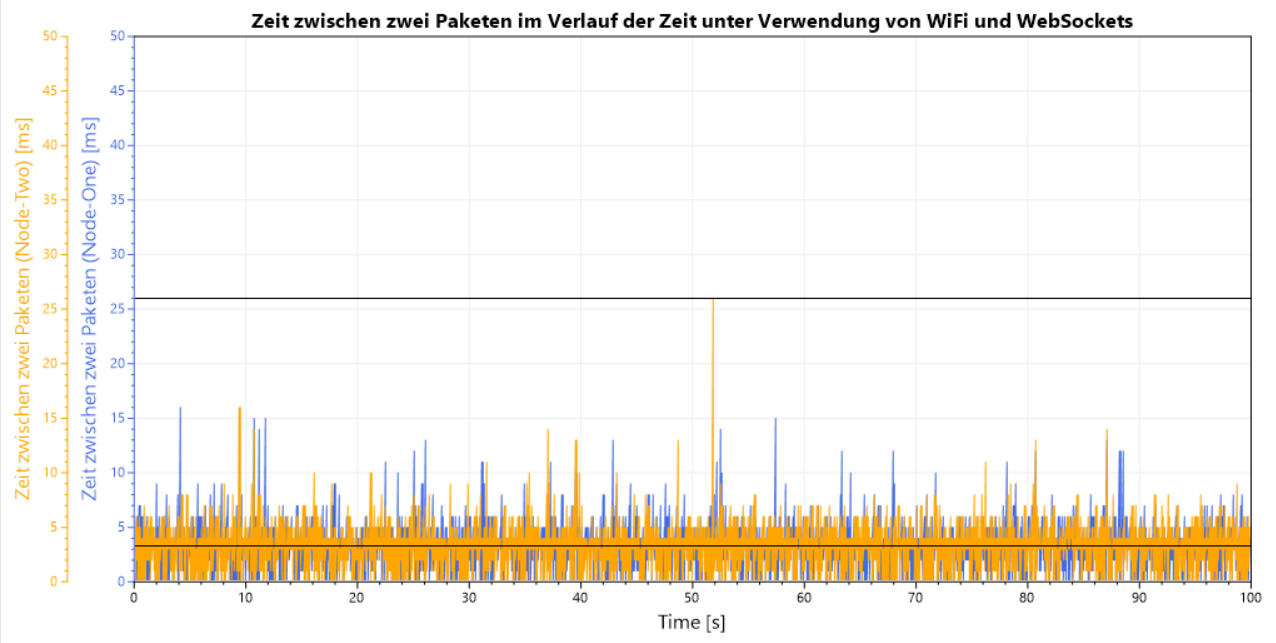
\includegraphics[width=\textwidth]{wifiStats.PNG}
    \caption{Intervall zwischen Paketen im Verlauf der Zeit bei WiFi}
    \label{fig:wifiStats}
\end{figure}
\begin{figure}[h]
    \centering
    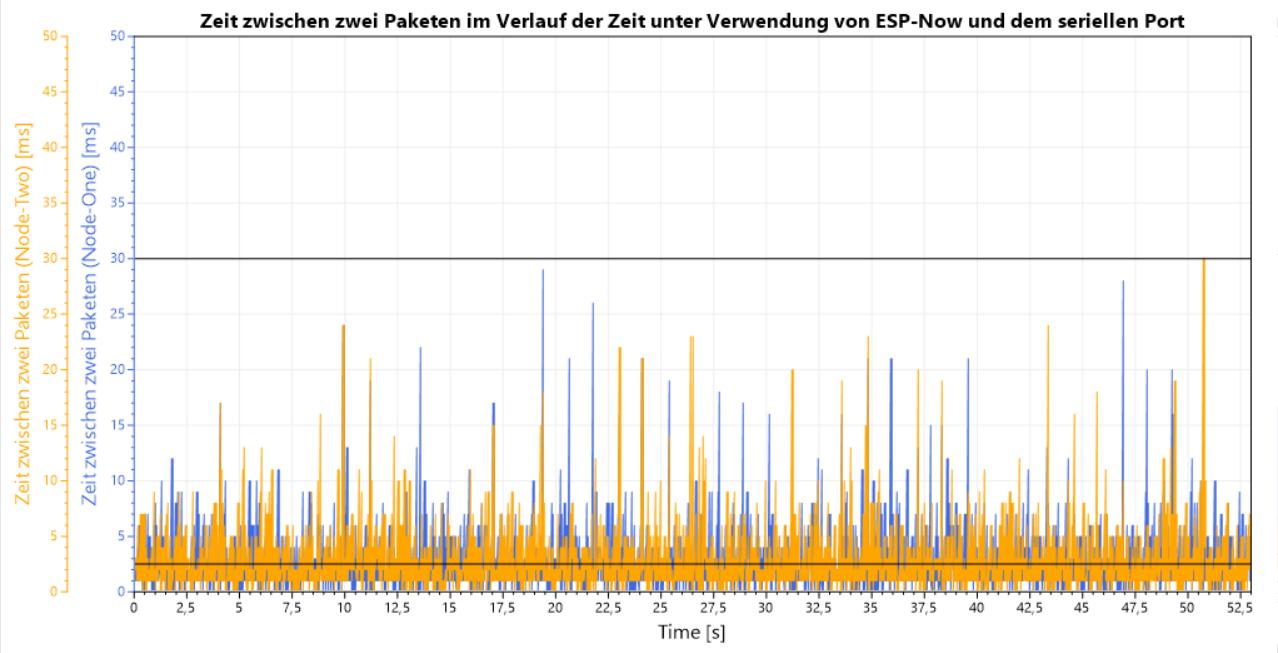
\includegraphics[width=\textwidth]{espnowStats.PNG}
    \caption{Intervall zwischen Paketen im Verlauf der Zeit bei ESP-Now}
    \label{fig:espnowStats}
\end{figure}

\begin{table}[h]
    \centering
    \begin{threeparttable}
        \caption{Messungen der getesteten Verbindungsmethoden}
        \begin{tabular}{|l|l|l|}
            \hline
            ~                                                                 & \parbox[c][1.5cm]{2cm}{\textbf{WiFi          \\mit\\WebSocket}} & \parbox[c][1.5cm]{2.5cm}{\textbf{ESP-Now\\mit\\seriellem Port}} \\ \hline
            \parbox[c][0.5cm]{6cm}{\textbf{Pakete pro Sekunde Durchschnitt} } & 250,16                              & 330,43 \\ \hline
            \parbox[c][0.5cm]{6cm}{\textbf{Pakete pro Sekunde Minimum}      } & 220                                 & 204    \\ \hline
            \parbox[c][0.5cm]{6cm}{\textbf{Pakete pro Sekunde Maximum}      } & 284                                 & 440    \\ \hline
            \parbox[c][0.5cm]{6cm}{\textbf{Paketintervall Durchschnitt [ms]}} & 3,09                                & 2,52   \\ \hline
            \parbox[c][0.5cm]{6cm}{\textbf{Paketintervall Minimum [ms]}     } & <1                                  & <1     \\ \hline
            \parbox[c][0.5cm]{6cm}{\textbf{Paketintervall Maximum [ms]}     } & 26                                  & 30     \\ \hline
        \end{tabular}
        \label{tab:connectionStats}
    \end{threeparttable}
\end{table}

Den Abbildungen \ref{fig:wifiStats} und \ref{fig:espnowStats}, sowie der Tabelle \ref{tab:connectionStats} ist zu entnehmen, dass das Interval zwischen zwei Paketen, bei beiden Mehtoden, im Schnitt im niedrigen einstelligen Millisekundenbereich ist.
ESP-Now mit seriellem Port schafft dabei im Durchschnitt 80 Pakete mehr als WiFi mit einem WebSocket.
Die Verbindung mit WiFi ist jedoch deutlich störungsfreier.
So ist aus Abbildung \ref{fig:espnowStats} abzulesen, dass entweder ESP-Now oder der serielle Port regelmäßiger, sowie höhere Ausreißer erzeugt, bei denen die Zeit zwischen zwei Paketen über 15 Millisekunden ist.
WiFi hingegen hat im kompletten Datensatz nur einen deutlichen Ausreißer (Abbildung \ref*{fig:wifiStats}) und hat ansonsten selten Zeiten über 15 Millisekunden. Es kann geschlussfolgert werden, dass WiFi vorzuziehen ist.
Jedoch kann auf ESP-Now mit seriellem Port zurückgegriffen werden, wenn nur ein \ac{usb}-Anschluss und kein WiFi Netzwerk verfügbar ist.
Anzumerken ist jedoch, dass die Messungen stark abhängig davon sind, welche \ac{usb}-Anschlüsse und -Protokolle verwendet wurden, sowie welche Datenraten der Router unterstützt.
Ein weiterer Einflussfaktor ist die Verbindung zwischen Client und dem Router.
Sind diese kabellos verbunden, erhöht sich zusätzlich die Zeit, die ein Paket zur Übertragung benötigt, im Gegensatz zur kabelgebundenen Übertragung.
Deshalb sind die erhobenen Messwerte nur begrenzt aussagekräftig.
Trotzdem lässt sich erkennen, dass beide Methoden genug Pakete verschicken können, um eine flüssige Bewegung nativ aus den Daten berechnen zu können.
Es sind keine Interpolationstechniken notwendig, um die Bewegung flüssig erscheinen zu lassen.

\newpage

\begin{table}
    \centering
    \caption{Die Verbindungsmethoden im Vergleich}
    \begin{tabular}{|l|l|l|}
        \hline
        ~                                                                                                                & \begin{tabular}[c]{@{}l@{}}\textbf{WiFi }\\\textbf{mit Websocket}\end{tabular}                                                           & \begin{tabular}[c]{@{}l@{}}\textbf{ESP-Now}\\\textbf{mit seriellem Port}\end{tabular}                                                    \\
        \hline
        \begin{tabular}[c]{@{}l@{}}\textbf{Anzahl }\\\textbf{Mikrocontroller}\end{tabular}                               & 2                                                                                                                                        & 3                                                                                                                                        \\
        \hline
        \textbf{Daten-Pfad}                                                                                              & \multicolumn{1}{c|}{\begin{tabular}[c]{@{}c@{}}ESP32\\↓\\Router\\↓\\Rollstuhl-Software\end{tabular}}                                     & \multicolumn{1}{c|}{\begin{tabular}[c]{@{}c@{}}ESP32\\↓\\ESP32\\↓\\Serieller Port\\↓\\Rollstuhl-Software\end{tabular}}                   \\
        \hline
        \begin{tabular}[c]{@{}l@{}}\textbf{"Hardcoding"}\\\textbf{von Verbindungs}\\\textbf{-informationen}\end{tabular} & nicht notwendig                                                                                                                          & Ziel-MAC-Adressen                                                                                                                        \\
        \hline
        \textbf{Vorteile}                                                                                                & \begin{tabular}{@{\labelitemi\hspace{\dimexpr\labelsep+0.5\tabcolsep}}l@{}}\begin{tabular}[c]{@{}l@{}}Stabile \\Verbindung\end{tabular}\\\begin{tabular}[c]{@{}l@{}}Nur eine \\Übertragungstechnologie\\notwendig\end{tabular}\end{tabular} & \begin{tabular}{@{\labelitemi\hspace{\dimexpr\labelsep+0.5\tabcolsep}}l@{}}\begin{tabular}[c]{@{}l@{}}Kein Verbinungsaufbau \\mit lokalem Netzwerk\\notwendig\end{tabular}\\\begin{tabular}[c]{@{}l@{}}Kein WiFi-Netzwerk \\notwendig, ein \\USB-Anschluss genügt\end{tabular}\end{tabular} \\
        \hline
    \end{tabular}
\end{table}